% !TEX root=template.tex

\typeout{NT FILE tests.tex}

\prependtographicspath{{Chapters/Figures/}}

\chapter{Tests}
\label{cha:tests}

With the implementation done, it is time to test the system. First, a few performance tests were executed to ascertain the efficiency of the \acrlong{ME} when compared to a standard implementation. Agent deployment times and skill execution times were measured and compared. A brief explanation of the physical system used to simulate a production line is given. Then the tests on this system are described. Finally, a few deployment and skill execution tests are described to ascertain the efficiency of the \acrshort{ME}.

\section{Performance Tests}
\label{sec:performance_tests}

The performance tests were done on a machine with an AMD Ryzen 7 5700X processor and 32 gigabytes of RAM.

\subsection{Deployment Test}

The first test is the deployment test. In it, an increasingly amount of agents are launched to measure how long it takes to launch each agent. An agent using the \acrlong{ME} and a normal agent are compared to ascertain how much the \acrshort{ME} impacts agent launch times.

This test was repeated three times, the first a single agent of each type is launched, the second ten agents of each type are launched, and the third a hundred agents are launched. Measurements are made by starting a timer when the "setup" method of an agent starts, and then stopped once the setup finishes. An agent running the \acrlong{ME} should take longer since it needs to get the parameters from the deployment entity and needs to instantiate its \acrshort{ME} and wait for the \acrshort{LL} loads before it finishes setup. The comparison is made between an agent that needs to follow these procedures versus and agent that does not. The times are written to a file that gets read to extract the values and calculate results.

As expected, and agent using the \acrshort{ME} takes more time before it is ready to operate. The single agent took around 15 milliseconds to launch. An agent without the \acrshort{ME} took around 0.0016 milliseconds.

Ten agents with the \acrshort{ME} took 17.5 milliseconds total, with an average time of 1.75 milliseconds for each agent while the agents without took 0.0018 milliseconds total, with an average of 0.00018 milliseconds per agent. 

Finally, a hundred agents with \acrshort{ME} needed 799 milliseconds, with an average time of 7.99 milliseconds per agent. The other agents needed 0.0658 milliseconds, with 0.000658 milliseconds per agent.

Although the launch times increased considerably, it must be taken into account that the agents with the \acrlong{ME} had a longer setup. This involves getting all the parameters needed to operate, instantiating the \acrshort{ME}, finding and loading the \acrshort{LL}. Even though the time it takes for setup to complete is higher, for an agent making use of the \acrshort{ME}, it is still under acceptable values for deployment, since none have too great a magnitude.

\begin{table}[h!]
	\caption{Deployment times.}
	\centering
	\begin{tabular}{|c|cc|cc|}
		\hline
		\multirow{2}{*}{Number of agents} & \multicolumn{2}{c|}{with Module Engine} 				& \multicolumn{2}{c|}{without Module Engine} \\ \cline{2-5} 
										  & \multicolumn{1}{c|}{Total}   	  & Average  			& \multicolumn{1}{c|}{Total}      			& Average  	  \\ \hline
		1                                 & \multicolumn{1}{c|}{15 ms}        & 15 ms               & \multicolumn{1}{c|}{0.0016 ms}    		& 0.0016 ms   \\ \hline
		10                                & \multicolumn{1}{c|}{1.75 ms}      & 17.5 ms             & \multicolumn{1}{c|}{0.0018 ms}    		& 0.00018 ms  \\ \hline
		100                               & \multicolumn{1}{c|}{799 ms}       & 7.99 ms             & \multicolumn{1}{c|}{0.0658 ms}  			& 0.000658 ms \\ \hline
	\end{tabular}
	\label{tab:deployment_times}
\end{table}

\subsection{Execution Test}

The second test is the skill execution delay test. Here, a skill is executed through the \acrlong{ME}. A special \acrlong{LL} was developed for this test, and its only function is to return a String to simulate the result of a skill. This result is then written on the console. The execution time of this operation is compared to the time it takes for the system to write the same message to the console, without going through the \acrshort{ME}.\\

This test was repeated sixty times, the five best and worst results excluded from the measured values to control for variations. The average time was calculated and compared. The operation without the \acrshort{ME} takes an average time of 0.012576 milliseconds. The operation with the \acrshort{ME} takes an average time of 0.028976 milliseconds, also less than a millisecond.\\

The difference between executing with the \acrshort{ME} is around 0.0164 milliseconds, when compared to executing without. It takes almost double the time for the message to be written. This was expected since there are more operations occurring with the \acrshort{ME}. Even though execution time does increase, it still is well under a millisecond, so the impact caused by the \acrlong{ME} and \acrlongpl{LL} is not huge, making it a viable option for most applications.

\begin{table}[h!]
	\centering
	\caption{Execution times.}
	\begin{tabular}{l|c|c|}
		\cline{2-3}
									& with Module Engine & without Module Engine \\ \hline
		\multicolumn{1}{|l|}{Time} 	& 0.028976 ms           & 0.012576 ms              \\ \hline
	\end{tabular}
	\label{tab:execution_times}
\end{table}

\section{Case Study}

The \acrshort{MAS} was simulated on a physical system composed of a conveyor belt and two processing stations. The conveyor belt is divided into four sections, each with their own sensor. This means that products can stop in the middle of any of the four sections. They are also independent, meaning that they can move and stop individually. The stations can move forward, backward, up and down, and their tool spins to simulate the execution of a skill. This model is illustrated in Figure~\ref{fig:physical_system}.

\begin{figure}[h!]
	\centering
	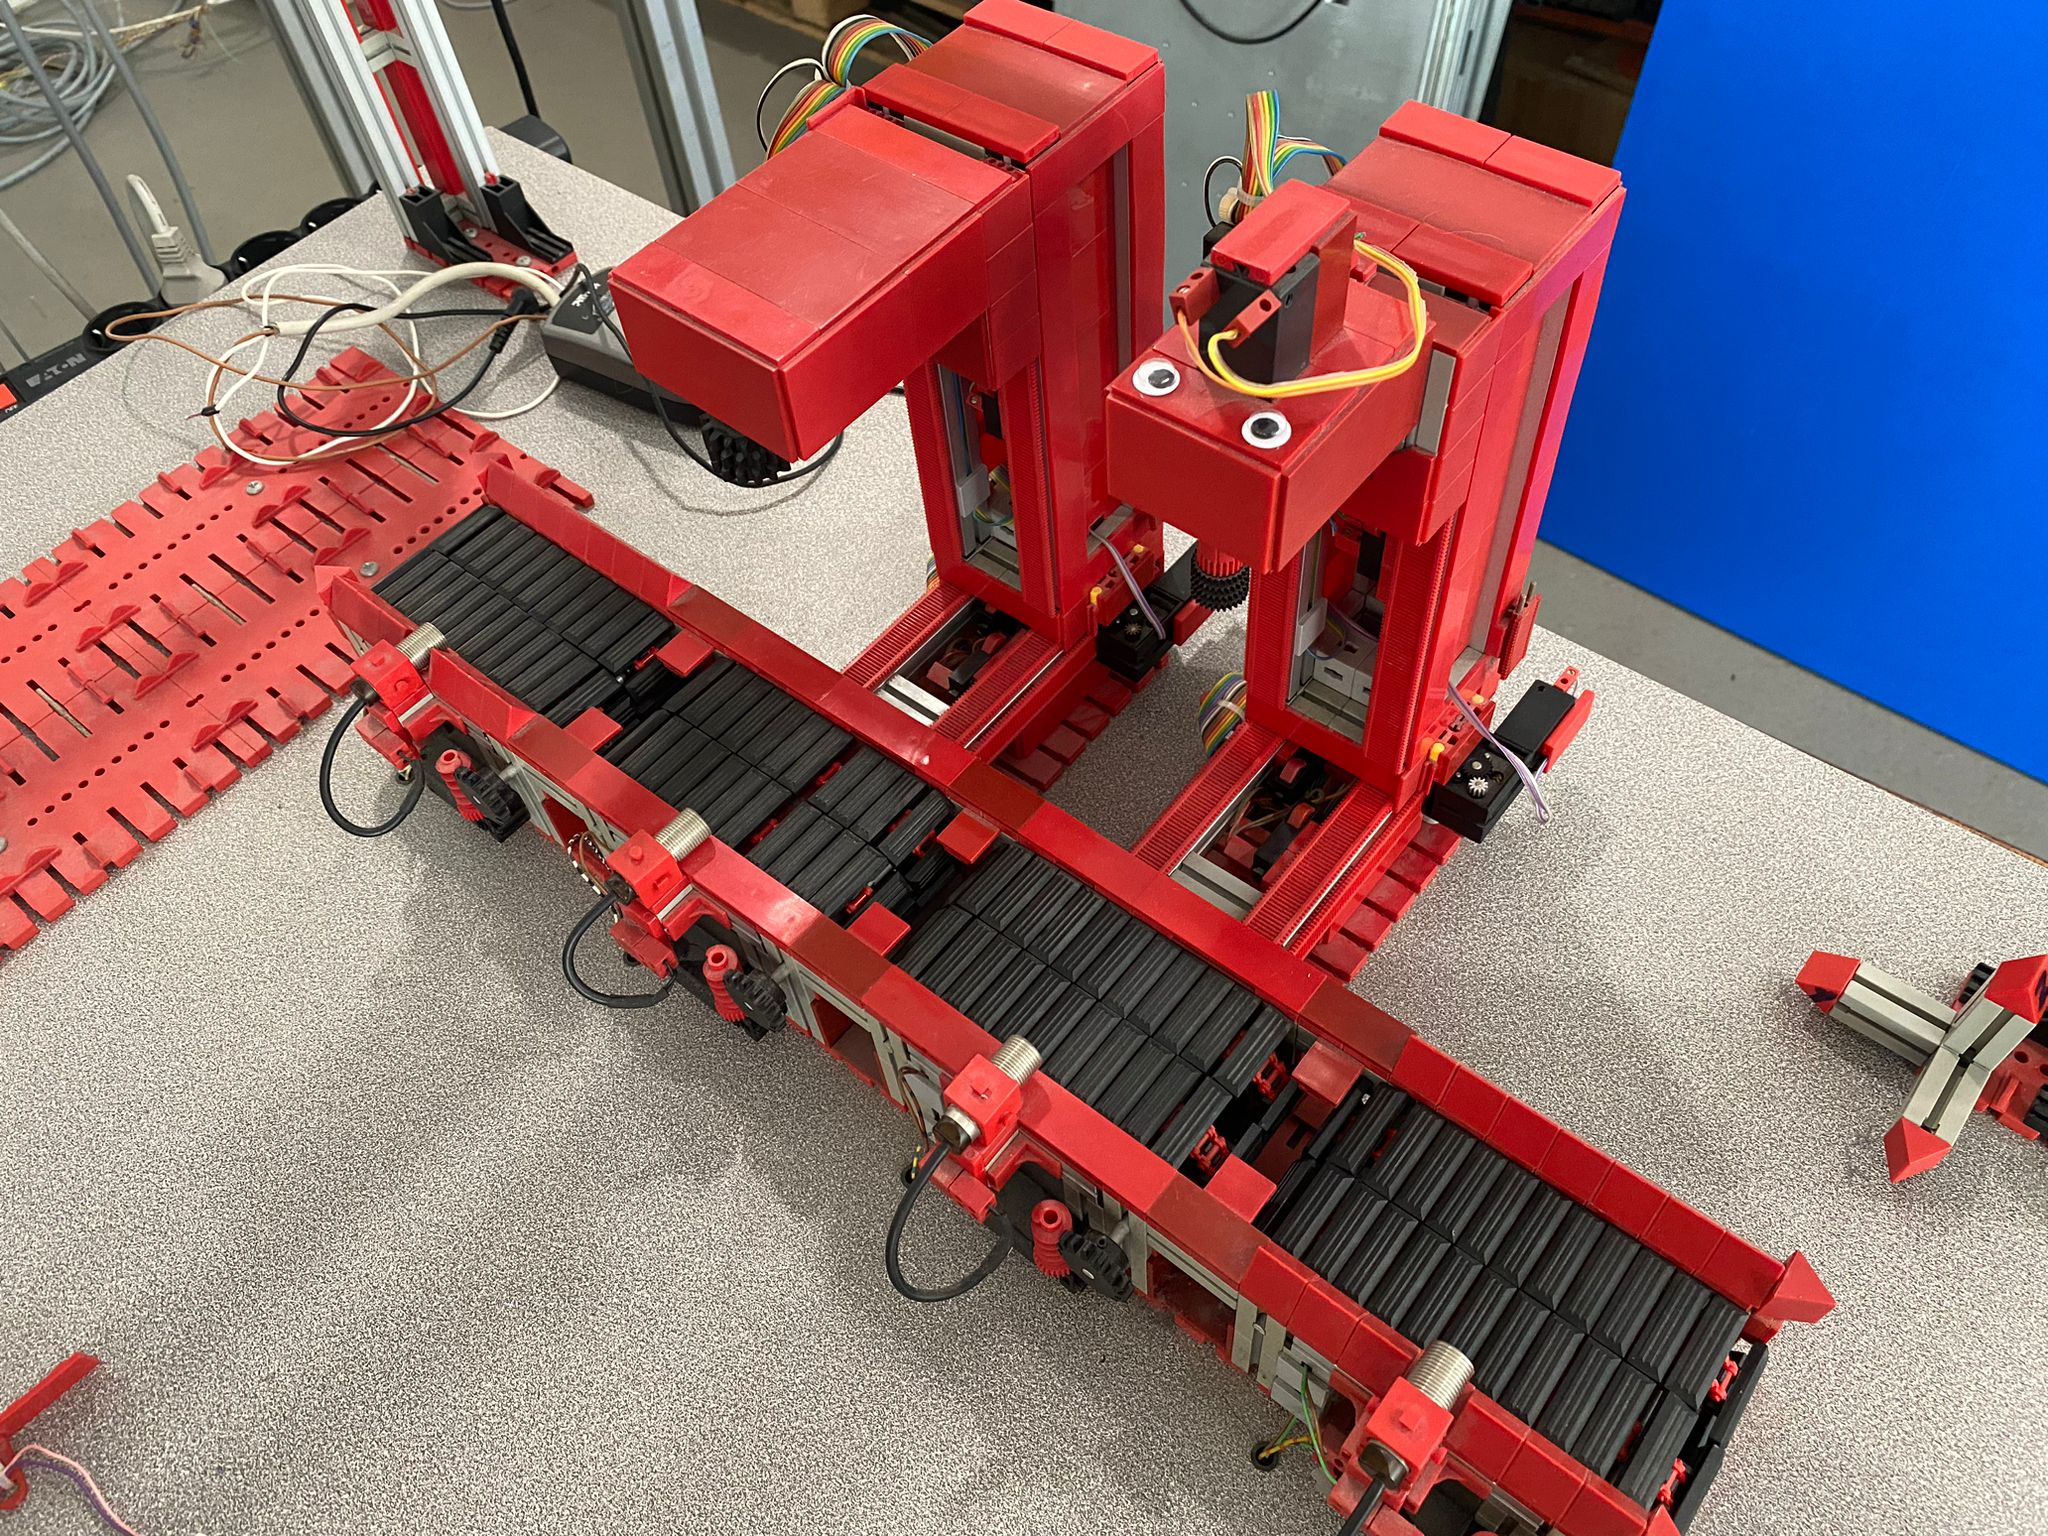
\includegraphics[scale=0.15]{Lateral_top_view.jpeg}
	\caption{Simulation kit.}
	\label{fig:physical_system}
\end{figure}

Each element of this system can be represented by an agent. The conveyor belt fits the definition of a \acrlong{TA} and both stations can be \acrlong{RA}. All of these entities were defined in the "Constants" class, the \acrshort{TA} as "Conveyor" and both stations as "Station\_3", for the station on the left (Figure~\ref{fig:station_3}), and "Station\_4", for the station on the right (Figure~\ref{fig:station_4}). 

Both stations are able to perform a skill. To reduce complexity, each station was attributed a single unique skill. "Station\_3" is able to perform "Skill\_A" and "Station\_4" can perform "Skill\_B". Both of these were also defined in the "Constants" class. These skills are registered by the respective agent in the \acrshort{DF}. The act of performing the skill corresponds to the device moving forward, activating its tool for about three seconds and then moving to the starter position.\\

\begin{figure}[h!]
	\centering
	\subbottom[Station 3.\label{fig:station_3}]{%
		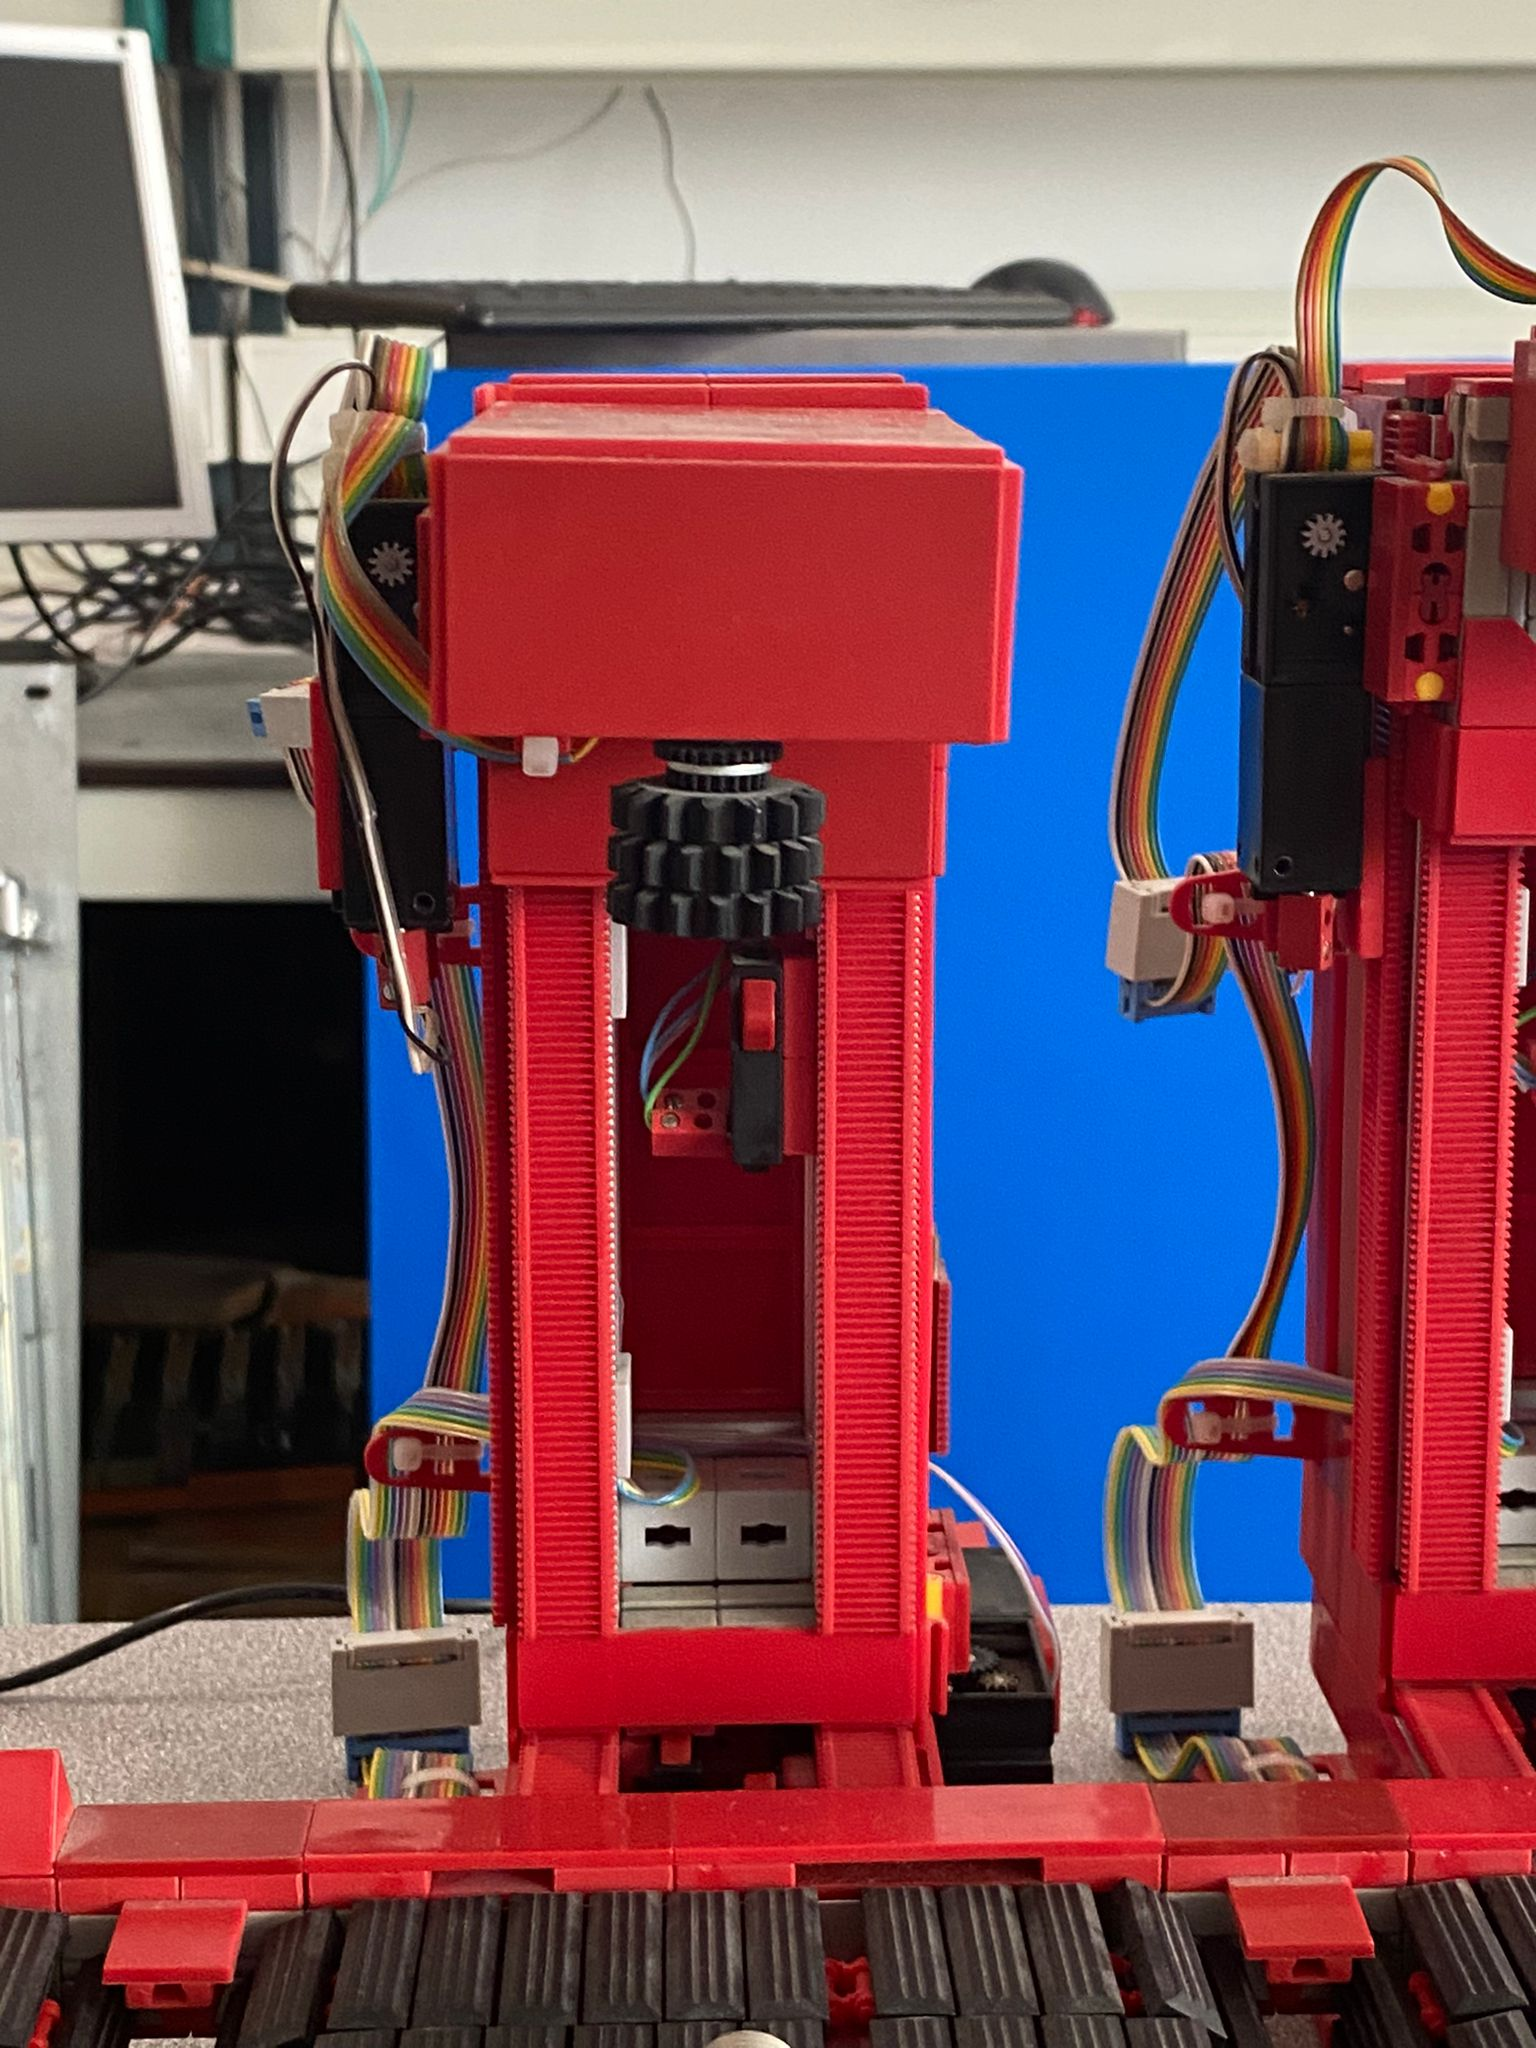
\includegraphics[width=0.35\linewidth]{Station_3.jpeg}}%
	\hspace{0.80cm}
	\subbottom[Station 4.\label{fig:station_4}]{%
		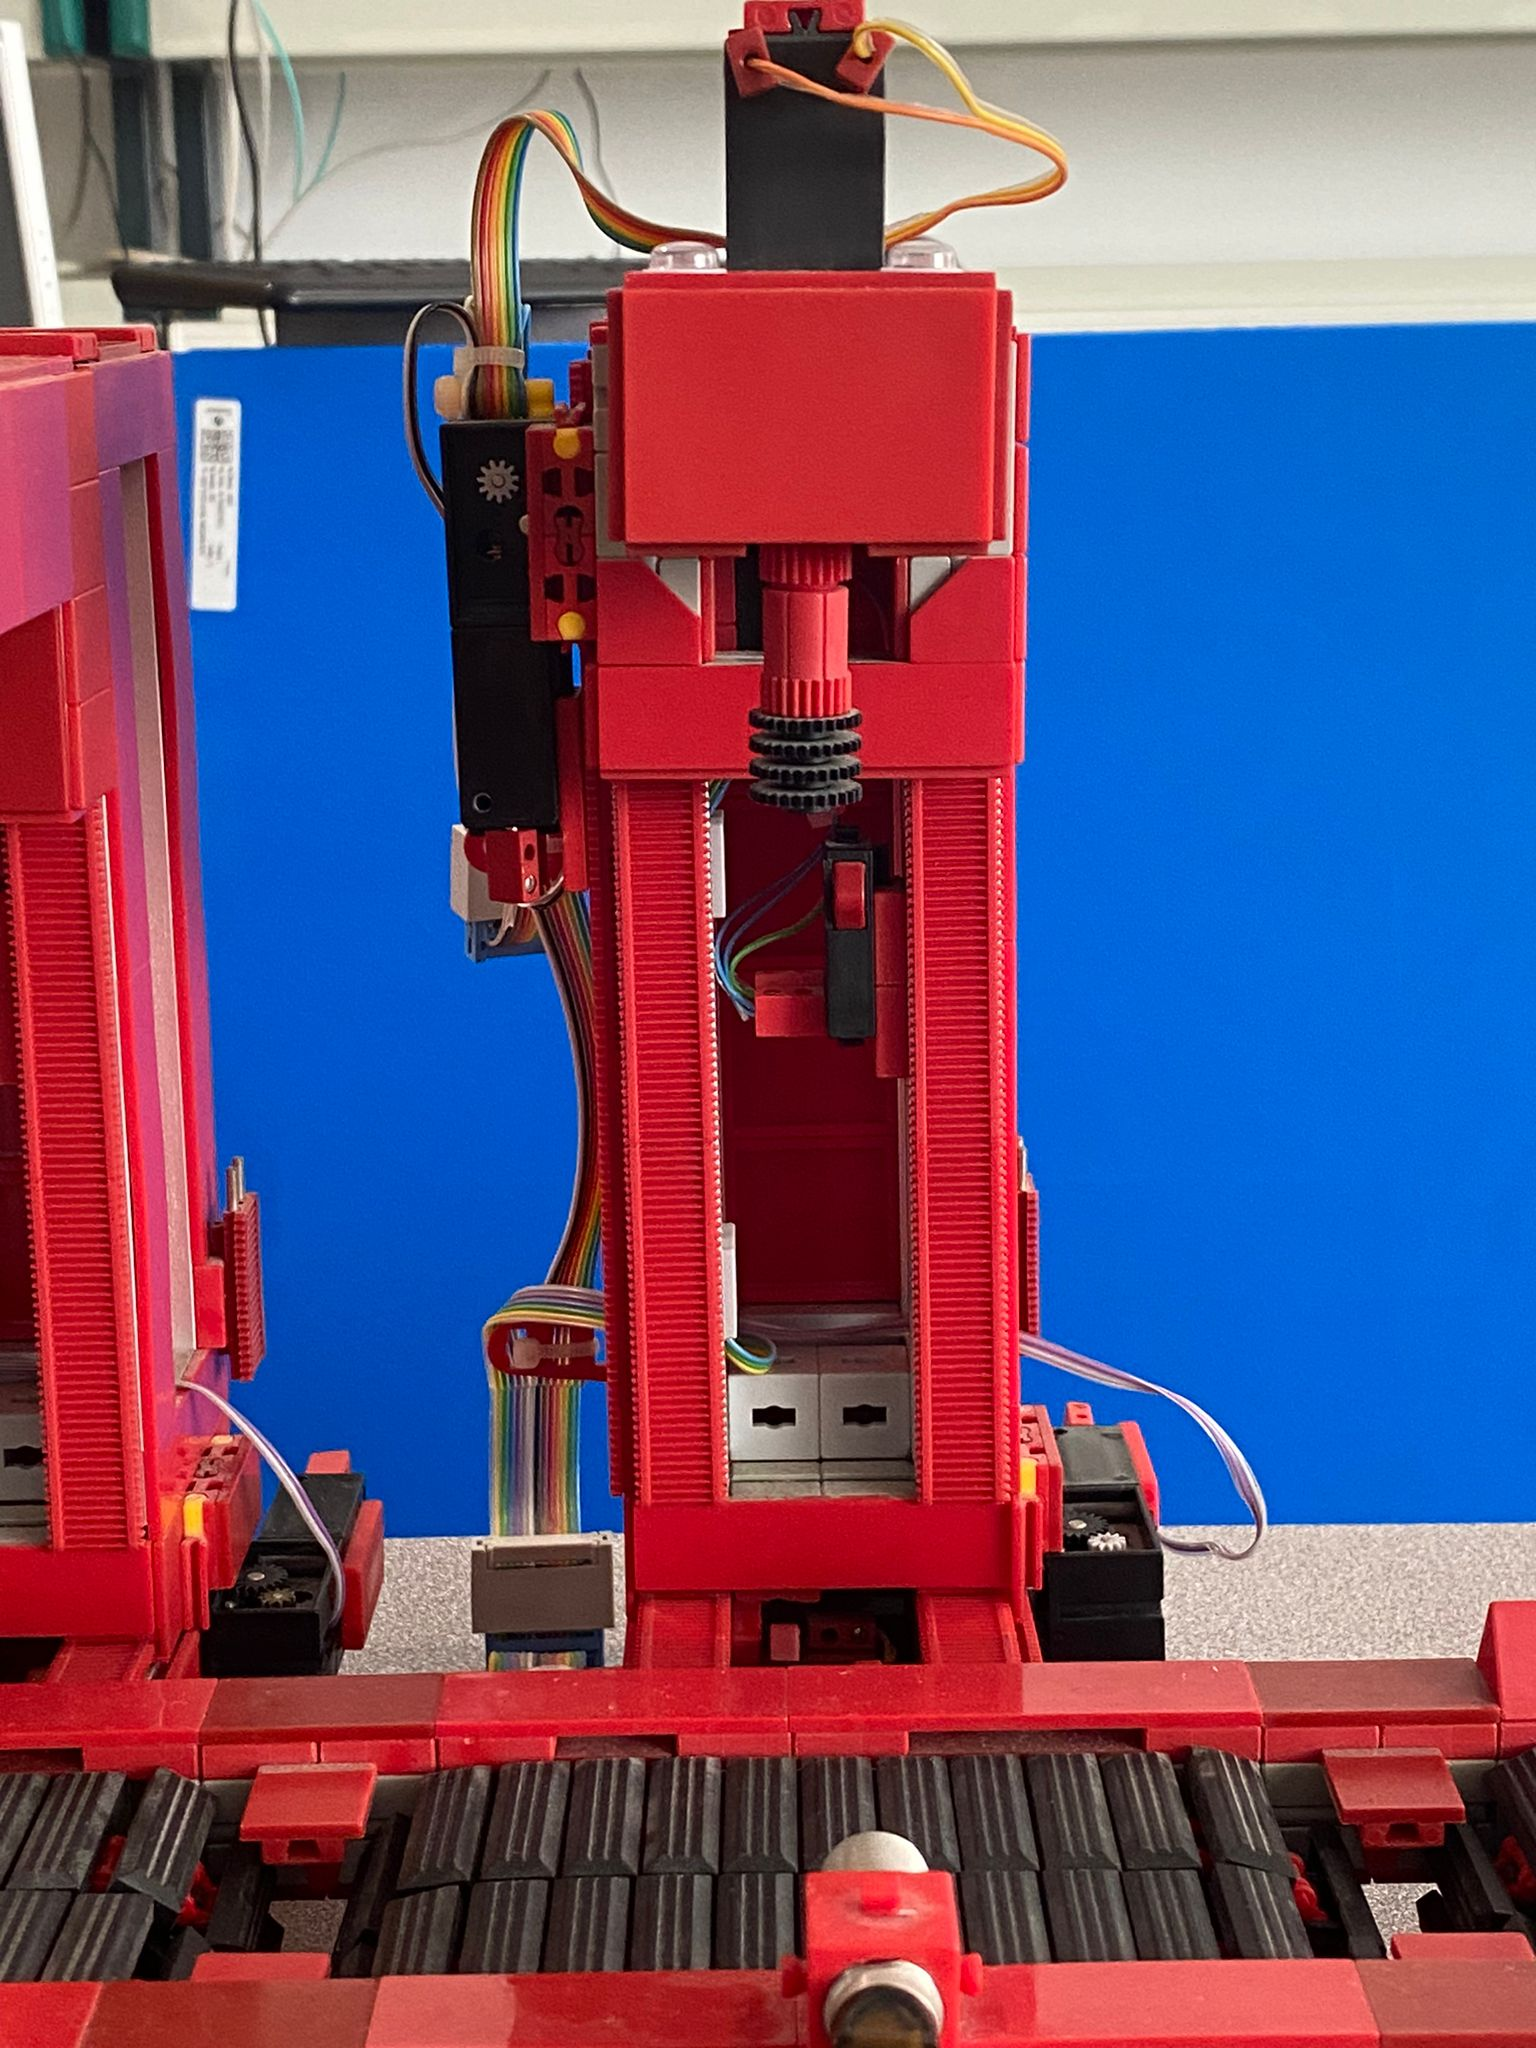
\includegraphics[width=0.35\linewidth]{Station_4.jpeg}}%
	\caption{Kit stations.}
	\label{fig:stations}
\end{figure}

The "Conveyor" agent is capable of performing the skill "Skill\_Move", also defined in the "Constants". This is the skill with which the agent registers itself in the \acrshort{DF}. When a \acrlong{PA} needs transportation, it must send a message to the "Conveyor" agent through the aforementioned channels in the format "CX\#TOKEN\#CY". Here, X represents the source location and Y represents the destiny location. The conveyor is split into four segments, numbered one to four from the left to the right. Each segment has a sensor that detects whether or not a product is on it. So the instruction "C1\#TOKEN\#C3" makes the conveyor turn the first, second and third segments to the right. Similarly, the instruction "C3\#TOKEN\#C2" makes the conveyor turn the second and third segments to the left.\\

A RevPi running an instance of NodeRED was used to control the system, its inputs and outputs connected to the conveyor and stations. A RevPi is a Raspberry Pi equipped with an shield board that allows it to interface hardware, like sensors and actuators. This RevPi was hosting the NodeRED instance, and it depended on an official RevPi NodeRED library to control the physical system.\\

NodeRED is an open source programming tool, capable of integrating hardware. It works by connecting nodes, which send messages to other connected nodes to complete processes. These groupings of nodes are called flows. Three flows were created, one for each cyber-physical entity. These flows are capable of receiving messages in \acrshort{HTTP}, \acrshort{MQTT} and \acrshort{OPCUA}, and return the result through the same protocol. Figure~\ref{fig:nodered_flows} shows the developed nodes. It also shows the \acrshort{OPCUA} server that was needed for \acrshort{OPCUA} communications. The \acrshort{MQTT} broker was hosted on a different machine.\\

\begin{figure}[h!]
	\centering
	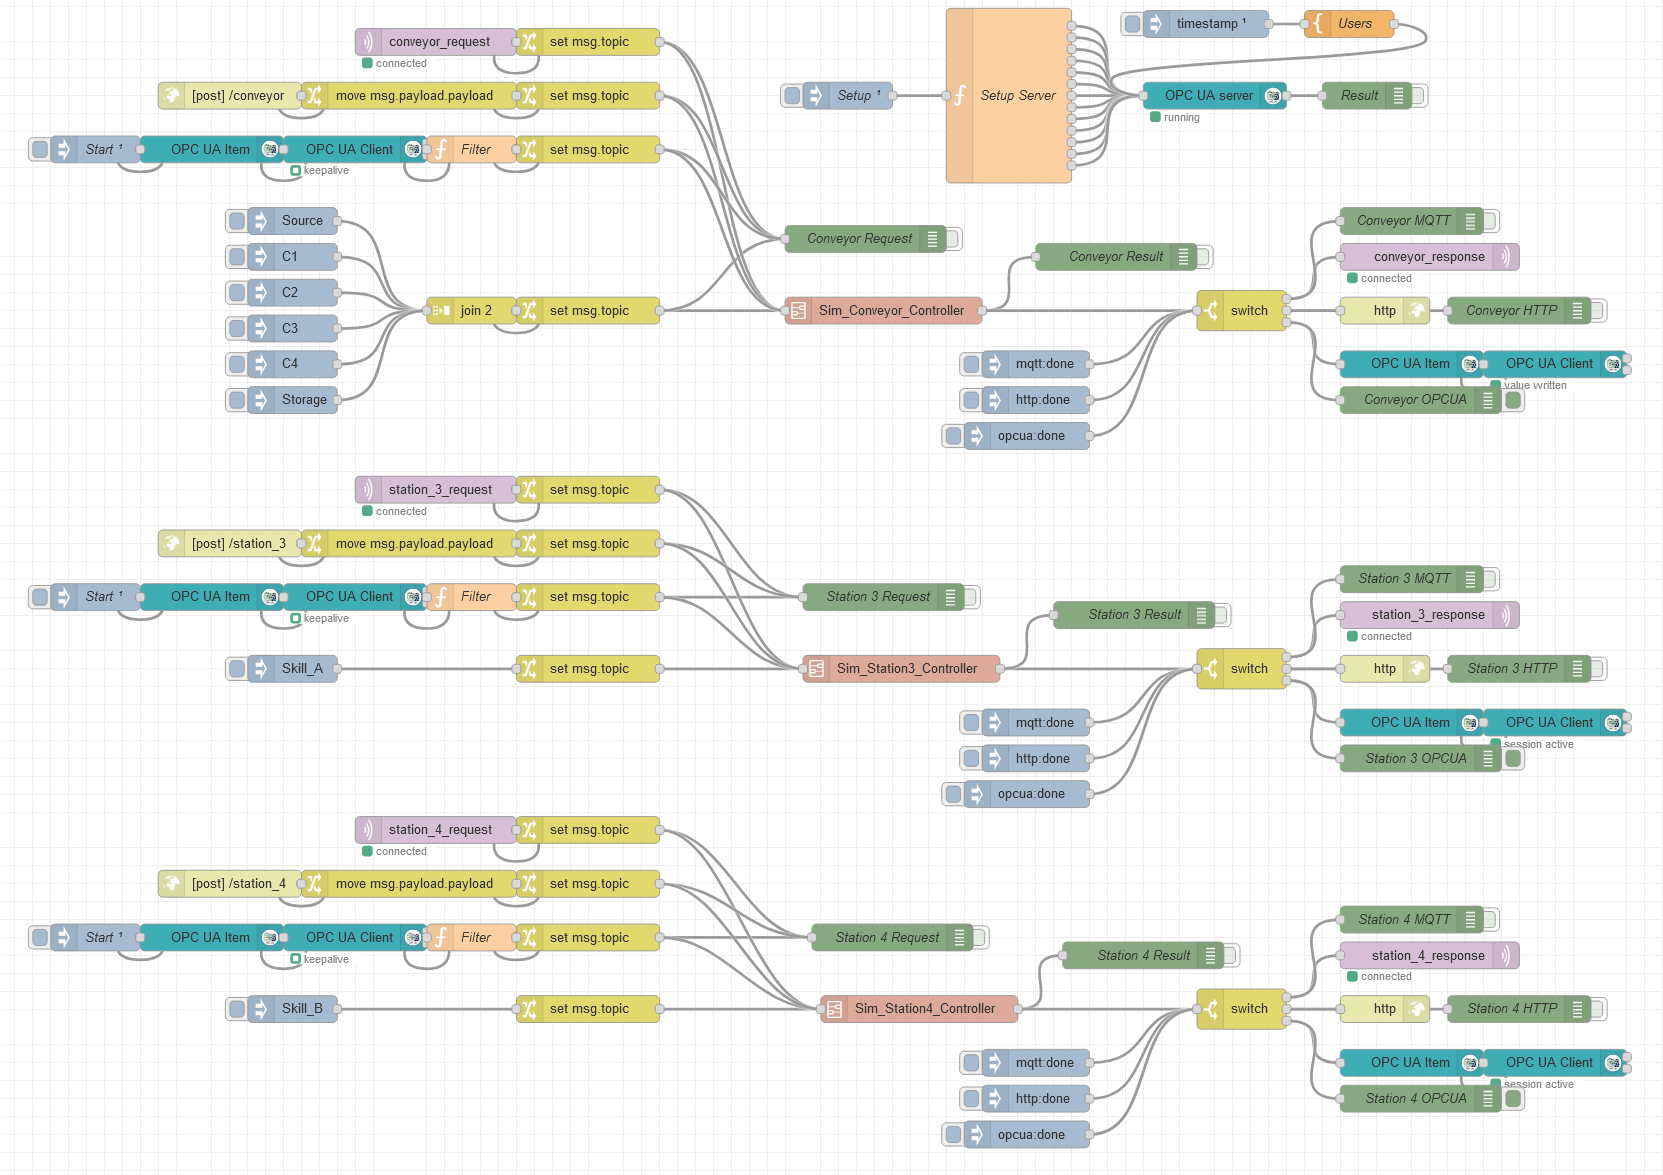
\includegraphics[scale=0.3]{NodeRED_flows.png}
	\caption{NodeRED flows.}
	\label{fig:nodered_flows}
\end{figure}

Three configuration files were created, one for each cyber-physical entity. A single file contains the configurations needed for the three developed \acrlongpl{LL}. Table~\ref{tab:mqtt_config} shows the configurations for the \acrshort{MQTT} protocol and Table~\ref{tab:opcua_config} for \acrshort{OPCUA}. The address field is not shown as well as the configurations for \acrshort{HTTP} since the only element therein is the server address.

\begin{table}[h!]
	\centering
	\caption{\acrshort{MQTT} configurations.}
	\begin{tabular}{c|c|c|c|}
		\cline{2-4}
		& Station\_3                 & Station\_4                 & Conveyor                   \\ \hline
		\multicolumn{1}{|c|}{Quality of Service} & 2                 		& 2                          & 2                          \\ \hline
		\multicolumn{1}{|c|}{Request topic}      & station\_3\_request        & station\_4\_request        & conveyor\_request          \\ \hline
		\multicolumn{1}{|c|}{Response topic}     & station\_3\_response       & station\_4\_response       & conveyor\_response         \\ \hline
	\end{tabular}
	\label{tab:mqtt_config}
\end{table}

\begin{table}[h!]
	\centering
	\caption{\acrshort{OPCUA} configurations.}
	\begin{tabular}{c|c|c|c|}
		\cline{2-4}
		& Station\_3    & Station\_4    & Conveyor      \\ \hline
		\multicolumn{1}{|c|}{Namespace index}     & 1             & 1             & 1             \\ \hline
		\multicolumn{1}{|c|}{Requests identifier} & Station3\_Req & Station4\_Req & Conveyor\_Req \\ \hline
		\multicolumn{1}{|c|}{Response identifier} & Station3\_Res & Station4\_Res & Conveyor\_Res \\ \hline
	\end{tabular}
	\label{tab:opcua_config}
\end{table}

To simulate the system, both NodeRED and the \acrshort{MAS} systems were launched. The \acrlong{PM} and \acrlong{DA} are immediately deployed, finish their initial setup explained in \ref{subsec:initial_setup} and wait for agents to be launched. After this, the two \acrlongpl{RA} were launched through the \acrshort{GUI}, "Station\_3" and "Station\_4", with their respective configurations. Along with those agents, the "Conveyor" \acrlong{TA} is also launched, also with its configuration file. At first, all agents are using the \acrshort{LL} that communicates through \acrshort{MQTT}, and thus the configurations for this protocol are used. These agents are connected to the broker on launch, and will communicate to the corresponding topics.\\

After the agents were done with their initial setups, a product agent was launched. For the purposes of showcasing the systems capabilities, three different Product Types were created. These products are shown in \ref{tab:product_types}, along with their production sequences and the sequence of Conveyor Belt sections they need to visit in order to complete their process. All of these values were also defined in the "Constants" class.

\begin{table}[h!]
	\caption{Product Types.}
	\centering
	\begin{tabular}{|c|c|c|}
		\hline
		Product Type & Production Sequence      & Location Sequence    \\ \hline
		A            & {[}Skill\_A{]}           & {[}C1; C2; C4{]}     \\ \hline
		B            & {[}Skill\_B{]}           & {[}C1; C3; C4{]}     \\ \hline
		C            & {[}Skill\_B; Skill\_A{]} & {[}C1; C3; C2; C4{]} \\ \hline
	\end{tabular}
	\label{tab:product_types}
\end{table}

All three product types were launched, one at a time. Product A was first, and the system was able to complete the production sequence without any problems. The product first went to Station 3, the station applied the skill, and then moved on to storage. The other two products followed a similar result, their production sequence executed as planned. This means the \acrlong{ME} was working as intended. Even though it wasn't hard-coded to the \acrshort{MQTT} protocol, it was able to use the \acrlong{LL} that integrates it to communicate to the machines.

To further test the \acrshort{ME}, "Station\_3" was taken down and restarted, this time with the \acrshort{HTTP} \acrlong{LL}. The same procedure was performed, with the same result. No noticeable difference was observed in the three products sequences. The \acrshort{ME} was once again integrating a new protocol.

The only difference noted was when \acrshort{OPCUA} was used, the stations wouldn't respond as fast to the instructions. However, this was attributed to the fact that the RevPi was running both the \acrshort{OPCUA} server and the NodeRED instance, overloading its processor. This could easily explain the delay observed. Despite this, the \acrshort{ME} was also capable of integrating this protocol.\\

Many combinations of the three protocols were used, with the same results. The \acrlong{ME} was integrating all three protocols as if it was hard-coded with them. The \acrlongpl{LL} developed were acting as interfaces between the \acrshort{ME} and NodeRED, but this interface could be replaced at any point to integrate new hardware.

This outcome was expected, since through the use of the Reflections feature of the Java programming language, a class can be loaded during runtime as if the program was compiled with it. Some kind of delays were to be expected, since there are extra instructions running in the background due to the \acrlong{ME} serving as an intermediary between agent and \acrlong{LL}, but their impact is minimal, since the \acrshort{ME} is fairly lightweight.